\begin{frame}{Progettazione Concettuale}
\vspace{.5cm}
Lo sviluppo di un database di un'applicazione passa attraverso diverse fasi di progettazione:
\begin{itemize}[<+->]
    \item concettuale;
    \item logica;
    \item fisica.
\end{itemize}
\pause
\begin{block}{Progettazione concettuale}
    La \textbf{progettazione concettuale} \`e la sintesi tra la visione degli utenti e la visione dei progettisti dell'applicazione.
\pause
Deve possedere 2 caratteristiche:
    \begin{enumerate}[<+->]
        \item assolutamente \textbf{precisa}: per non lasciare dubbi sulle caratteristiche della base di dati che si sta progettando;
        \item deve essere espressa tramite \textbf{formalismi semplici} da permettere la lettura e la comprensione anche da parte di utenti non tecnici.
    \end{enumerate}
\end{block}
\end{frame}
%
\begin{frame}{Progettazione Concettuale}
\vspace{.4cm}
Il modello \textbf{Entit\`a/Associazioni} o \textbf{Entity/Relationships (ER)} ha queste caratteristiche e si concretizza in un documento con schemi grafici:
\pause
{\begin{center}
\begin{tikzpicture}[remember picture]
    % Define styles for shapes
    \tikzstyle{rectangle} = [draw, minimum width=3cm, minimum height=1cm]
    \tikzstyle{rhombus} = [draw, diamond, minimum width=3cm, minimum height=1cm, aspect=2]
    % Draw shapes
    \node[rectangle] (rect1) at (1.5, -1) {
            \begin{tabular}{c}
                \textbf{Fornitore} \\
                \hline
                CodFornitore (PK) \\
                Nominativo \\
                Via \\
                Citt\`a \\
                CAP \\
            \end{tabular}
    };
    \node[rhombus] (rhombus) at (7, -1) {Fornire};
    \node[rectangle] (rect2) at (12.5, -1) {
            \begin{tabular}{c}
                \textbf{Prodotto} \\
                \hline
                CodProdotto (PK) \\
                Descrizione \\
                Prezzo \\
            \end{tabular}
        };
     % Fornire rectangle under the rhombus
     \node[rectangle] (rect3) at (7, -4) {
        \begin{tabular}{c}
             \\
            \hline
            DataAcquisto \\
            Quantit\`a \\
        \end{tabular}
    };
    % Draw arrows
    \draw[dashed] (rect1) -- (rhombus) node[midway, above] {(1,N)};
    \draw (rhombus) -- (rect2) node[midway, above] {(1,N)};
     % line from rhombus to the Fornire rectangle
     \draw (rhombus) -- (rect3) node[midway, right] {};
\end{tikzpicture}
\end{center}}
\end{frame}
%
\begin{frame}{Progettazione Concettuale: alcune osservazioni}
\vspace{-.7cm}
\begin{center}
\begin{tikzpicture}[remember picture]
    % Define styles for shapes
    \tikzstyle{rectangle} = [draw, minimum width=3cm, minimum height=1cm]
    \tikzstyle{rhombus} = [draw, diamond, minimum width=3cm, minimum height=1cm, aspect=2]
    % Draw shapes
    \node[rectangle] (rect1) at (1.5, -1) {
            \begin{tabular}{c}
                \textbf{Fornitore} \\
                \hline
                CodFornitore (PK) \\
                Nominativo \\
                Via \\
                Citt\`a \\
                CAP \\
            \end{tabular}
    };
    \node[rhombus] (rhombus) at (7, -1) {Fornire};
    \node[rectangle] (rect2) at (11.5, -1) {
            \begin{tabular}{c}
                \textbf{Prodotto} \\
                \hline
                CodProdotto (PK) \\
                Descrizione \\
                Prezzo \\
            \end{tabular}
        };
     % Fornire rectangle under the rhombus
     \node[rectangle] (rect3) at (7, -3) {
        \begin{tabular}{c}
             \\
            \hline
            DataAcquisto \\
            Quantit\`a \\
        \end{tabular}
    };
    % Draw arrows
    \draw[dashed] (rect1) -- (rhombus) node[midway, above] {(1,N)};
    \draw (rhombus) -- (rect2) node[midway, above] {(1,N)};
     % line from rhombus to the Fornire rectangle
     \draw (rhombus) -- (rect3) node[midway, right] {};
\end{tikzpicture}
\end{center}
\begin{itemize}[<+->]
    \item Lo schema descrive i prodotti acquistati da un'impresa e i relativi fornitori.
    \item Pregio di questa rappresentazione: linguaggio naturale!
    
    Il modello permette di affermare che:
    \begin{itemize}
        \item ogni fornitore pu\`o fornire uno o pi\`u prodotti;
        \item ogni prodotto deve essere fornito da un solo fornitore.
    \end{itemize}
\end{itemize}
\end{frame}
%
\begin{frame}{Modello dei dati}
    \block{Modello dei dati}
        \textbf{Modellare i dati} significa costruire una rappresentazione semplificata della reallt\`a osservata o si un problema, individuandone gli elementi caratterizzanti e i legami intercorrenti tra essi.
    \endblock
\pause
La progettazione di un modello di dati avviene a livelli diversi di astrazione dal problema considerato.
\pause
Si parla di:

\begin{itemize}[<+->]
    \item livello concettuale;
    \item livello logico;
    \item livello fisico.
\end{itemize}
\end{frame}
%
\begin{frame}{Modello dei dati}
\begin{center}
    \begin{tikzpicture}[node distance=2cm, auto, >={Stealth[length=4mm, width=3mm]}]

        % Define styles for shapes
        \tikzstyle{level} = [rectangle, draw, minimum width=4cm, minimum height=1cm, text centered, font=\large]
    
        % Draw the three levels
        \node[level] (conceptual) {Livello concettuale};
        \node[level, below of=conceptual] (logical) {Livello logico};
        \node[level, below of=logical, ] (physical) {Livello fisico};
    
        % Draw arrows between levels
        \draw[->, line width=1mm] (conceptual) -- (logical);
        \draw[->, line width=1mm] (logical) -- (physical);
    
        % Place images to the right of each rectangle
        \node[right=1cm of conceptual] {
\includegraphics[width=1cm]{img/conceptual-level.png}};
        \node[right=1cm of logical] {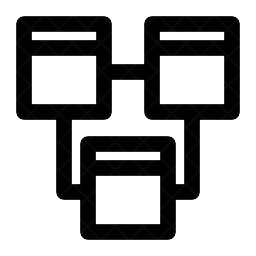
\includegraphics[width=1cm]{img/logical-level.png}};
        \node[right=1cm of physical] {
\includegraphics[width=1cm]{img/physical-level.png}};
        
    \end{tikzpicture}
\end{center}
\end{frame}
%
\begin{frame}{Livello concettuale}
\vspace{.5cm}
Il \textbf{livello concettuale} (o \textbf{livello di oggetti}) rappresenta la realt\`a dei dati e le relazioni tra essi attraverso uno schema.
\begin{center}
    \begin{tikzpicture}[node distance=2cm, auto, >={Stealth[length=4mm, width=3mm]}]

        % Define styles for shapes
        \tikzstyle{level} = [rectangle, draw, minimum width=4cm, minimum height=1cm, text centered, font=\large]
    
        % Draw the three levels
        \node[level, fill=red!30] (conceptual) {Livello concettuale};
        \node[level, below of=conceptual] (logical) {Livello logico};
        \node[level, below of=logical, ] (physical) {Livello fisico};
    
        % Draw arrows between levels
        \draw[->, line width=1mm] (conceptual) -- (logical);
        \draw[->, line width=1mm] (logical) -- (physical);
    
        % Place images to the right of each rectangle
        \node[right=1cm of conceptual] {
\includegraphics[width=1cm]{img/conceptual-level.png}};
        \node[right=1cm of logical] {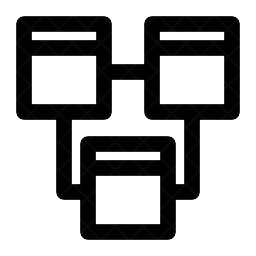
\includegraphics[width=1cm]{img/logical-level.png}};
        \node[right=1cm of physical] {
\includegraphics[width=1cm]{img/physical-level.png}};
        
    \end{tikzpicture}
\end{center}
\end{frame}
%
\begin{frame}{Livello logico}
Il \textbf{livello logico} (o \textbf{livello di record}) descrive come i dati sono organizzati negli archivi.

Esso descrive la composizione e il formato dei dati e la loro strutturazione logica.

Il livello logico viene derivato dal livello concettuale applicando alcune semplici regole di trasformazione.
\vspace{-.5cm}
\begin{center}
    \begin{tikzpicture}[node distance=2cm, auto, >={Stealth[length=4mm, width=3mm]}]

        % Define styles for shapes
        \tikzstyle{level} = [rectangle, draw, minimum width=4cm, minimum height=1cm, text centered, font=\large]
    
        % Draw the three levels
        \node[level] (conceptual) {Livello concettuale};
        \node[level, below of=conceptual, fill=red!30] (logical) {Livello logico};
        \node[level, below of=logical, ] (physical) {Livello fisico};
    
        % Draw arrows between levels
        \draw[->, line width=1mm] (conceptual) -- (logical);
        \draw[->, line width=1mm] (logical) -- (physical);
    
        % Place images to the right of each rectangle
        \node[right=1cm of conceptual] {
\includegraphics[width=1cm]{img/conceptual-level.png}};
        \node[right=1cm of logical] {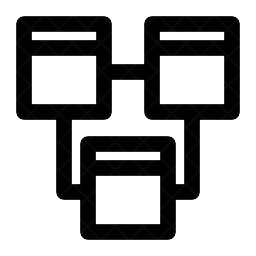
\includegraphics[width=1cm]{img/logical-level.png}};
        \node[right=1cm of physical] {
\includegraphics[width=1cm]{img/physical-level.png}};
        
    \end{tikzpicture}
\end{center}
\end{frame}
%
\begin{frame}{Livello fisico}
Il \textbf{livello fisico} rappresenta l'effettiva installazione degli archivi su disco.

Esso rappresenta l'implementazione del livellon logico sui supporti per la registrazione fisica dei dati e si occupa di oggetti quali: partizioni, puntatori, blocchi fisici, cluster, indici \ldots

\begin{center}
    \begin{tikzpicture}[node distance=2cm, auto, >={Stealth[length=4mm, width=3mm]}]

        % Define styles for shapes
        \tikzstyle{level} = [rectangle, draw, minimum width=4cm, minimum height=1cm, text centered, font=\large]
    
        % Draw the three levels
        \node[level] (conceptual) {Livello concettuale};
        \node[level, below of=conceptual] (logical) {Livello logico};
        \node[level, below of=logical, fill=red!30] (physical) {Livello fisico};
    
        % Draw arrows between levels
        \draw[->, line width=1mm] (conceptual) -- (logical);
        \draw[->, line width=1mm] (logical) -- (physical);
    
        % Place images to the right of each rectangle
        \node[right=1cm of conceptual] {
\includegraphics[width=1cm]{img/conceptual-level.png}};
        \node[right=1cm of logical] {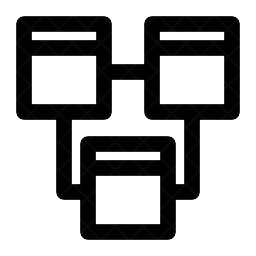
\includegraphics[width=1cm]{img/logical-level.png}};
        \node[right=1cm of physical] {
\includegraphics[width=1cm]{img/physical-level.png}};
        
    \end{tikzpicture}
\end{center}
\end{frame}
%
\begin{frame}{Dalla realt\`a agli archivi}
\begin{minipage}{0.35\linewidth}
\begin{tikzpicture}[node distance=2cm, auto, >={Stealth[length=4mm, width=3mm]}]
    % Define styles for shapes
    \tikzstyle{level} = [rectangle, draw, minimum width=4cm, minimum height=1cm, text centered, font=\large]
    
    % Draw the three levels
    \node[level] (reality) {Realt\`a};
    \node[level, below of=reality, fill=red!30] (conceptual) {Schema concettuale};
    \node[level, below of=conceptual] (logical) {Strutture logiche dei dati};
    \node[level, below of=logical] (physical) {Archivi};

    % Draw arrows between levels
    \draw[->, line width=1mm] (reality) -- (conceptual);
    \draw[->, line width=1mm] (conceptual) -- (logical);
    \draw[->, line width=1mm] (logical) -- (physical);
\end{tikzpicture}
\end{minipage}%
\begin{minipage}{0.65\linewidth}
\begin{block}{Schema concettuale}
    L'attivit\`a di progettazione richiede, prima di tutto, di costruire una rappresentazione astratta dalla realt\`a in modo indipendente dalla struttura dei dati.
    \pause
    \newline
    \\Il modello concettuale viene definito attraverso lo \textbf{schema} dei dati, cio\`e una rappresentazione sintetica (di solito in forma grafica) degli elementi fondamentali che caratterizzano la realt\`a osservata. 
    
    Questa \`e indipendente dai valori che verranno assegnati ai dati e alle applicazioni che utilizzano i dati.
\end{block}
\end{minipage}
\end{frame}
%
\begin{frame}{Dalla realt\`a agli archivi}
\begin{minipage}{0.35\linewidth}
\begin{tikzpicture}[node distance=2cm, auto, >={Stealth[length=4mm, width=3mm]}]
    % Define styles for shapes
    \tikzstyle{level} = [rectangle, draw, minimum width=4cm, minimum height=1cm, text centered, font=\large]
    
    % Draw the three levels
    \node[level] (reality) {Realt\`a};
    \node[level, below of=reality] (conceptual) {Schema concettuale};
    \node[level, below of=conceptual, fill=red!30] (logical) {Strutture logiche dei dati};
    \node[level, below of=logical] (physical) {Archivi};

    % Draw arrows between levels
    \draw[->, line width=1mm] (reality) -- (conceptual);
    \draw[->, line width=1mm] (conceptual) -- (logical);
    \draw[->, line width=1mm] (logical) -- (physical);
\end{tikzpicture}
\end{minipage}%
\begin{minipage}{0.65\linewidth}
\begin{block}{Strutture logiche dei dati}
    Con il passaggio al modello logico, l'insieme dei dati viene dotato di una struttura che deve facilitarne:
    \pause
    \begin{itemize}[<+->]
        \item la \textbf{manipolazione}: la possibilit\`a di inserire, modificare e cancellare i dati;
        \item l' \textbf{interrogazione}: la possibilit\`a di ritrovare i dati, richiesti da un'applicazione, in modo semplice e veloce.
    \end{itemize}
\end{block}
\end{minipage}
\end{frame}
%
\begin{frame}{Dalla realt\`a agli archivi}
\begin{minipage}{0.35\linewidth}
\begin{tikzpicture}[node distance=2cm, auto, >={Stealth[length=4mm, width=3mm]}]
    % Define styles for shapes
    \tikzstyle{level} = [rectangle, draw, minimum width=4cm, minimum height=1cm, text centered, font=\large]
    
    % Draw the three levels
    \node[level] (reality) {Realt\`a};
    \node[level, below of=reality] (conceptual) {Schema concettuale};
    \node[level, below of=conceptual] (logical) {Strutture logiche dei dati};
    \node[level, below of=logical, fill=red!30] (physical) {Archivi};

    % Draw arrows between levels
    \draw[->, line width=1mm] (reality) -- (conceptual);
    \draw[->, line width=1mm] (conceptual) -- (logical);
    \draw[->, line width=1mm] (logical) -- (physical);
\end{tikzpicture}
\end{minipage}%
\begin{minipage}{0.65\linewidth}
\begin{block}{Archivi}
    Queste strutture di dati vengono poi implementate sulle memorie di massa, realizzando in pratica il modello fisico, rappresentato dai file registrati nei blocchi del disco.
\end{block}
\end{minipage}
\end{frame}
%